
%% Beginning of file 'sample63.tex'
%%
%% Modified 2019 June
%%
%% This is a sample manuscript marked up using the
%% AASTeX v6.3 LaTeX 2e macros.
%%
%% AASTeX is now based on Alexey Vikhlinin's emulateapj.cls 
%% (Copyright 2000-2015).  See the classfile for details.

%% AASTeX requires revtex4-1.cls (http://publish.aps.org/revtex4/) and
%% other external packages (latexsym, graphicx, amssymb, longtable, and epsf).
%% All of these external packages should already be present in the modern TeX 
%% distributions.  If not they can also be obtained at www.ctan.org.

%% The first piece of markup in an AASTeX v6.x document is the \documentclass
%% command. LaTeX will ignore any data that comes before this command. The 
%% documentclass can take an optional argument to modify the output style.
%% The command below calls the preprint style which will produce a tightly 
%% typeset, one-column, single-spaced document.  It is the default and thus
%% does not need to be explicitly stated.
%%
%%
%% using aastex version 6.3
\documentclass{aastex63}
\usepackage{comment}
%% The default is a single spaced, 10 point font, single spaced article.
%% There are 5 other style options available via an optional argument. They
%% can be invoked like this:
%%
%% \documentclass[arguments]{aastex63}
%% 
%% where the layout options are:
%%
%%  twocolumn   : two text columns, 10 point font, single spaced article.
%%                This is the most compact and represent the final published
%%                derived PDF copy of the accepted manuscript from the publisher
%%  manuscript  : one text column, 12 point font, double spaced article.
%%  preprint    : one text column, 12 point font, single spaced article.  
%%  preprint2   : two text columns, 12 point font, single spaced article.
%%  modern      : a stylish, single text column, 12 point font, article with
%% 		  wider left and right margins. This uses the Daniel
%% 		  Foreman-Mackey and David Hogg design.
%%  RNAAS       : Preferred style for Research Notes which are by design 
%%                lacking an abstract and brief. DO NOT use \begin{abstract}
%%                and \end{abstract} with this style.
%%
%% Note that you can submit to the AAS Journals in any of these 6 styles.
%%
%% There are other optional arguments one can invoke to allow other stylistic
%% actions. The available options are:
%%
%%   astrosymb    : Loads Astrosymb font and define \astrocommands. 
%%   tighten      : Makes baselineskip slightly smaller, only works with 
%%                  the twocolumn substyle.
%%   times        : uses times font instead of the default
%%   linenumbers  : turn on lineno package.
%%   trackchanges : required to see the revision mark up and print its output
%%   longauthor   : Do not use the more compressed footnote style (default) for 
%%                  the author/collaboration/affiliations. Instead print all
%%                  affiliation information after each name. Creates a much 
%%                  longer author list but may be desirable for short 
%%                  author papers.
%% twocolappendix : make 2 column appendix.
%%   anonymous    : Do not show the authors, affiliations and acknowledgments 
%%                  for dual anonymous review.
%%
%% these can be used in any combination, e.g.
%%
%% \documentclass[twocolumn,linenumbers,trackchanges]{aastex63}
%%
%% AASTeX v6.* now includes \hyperref support. While we have built in specific
%% defaults into the classfile you can manually override them with the
%% \hypersetup command. For example,
%%
%% \hypersetup{linkcolor=red,citecolor=green,filecolor=cyan,urlcolor=magenta}
%%
%% will change the color of the internal links to red, the links to the
%% bibliography to green, the file links to cyan, and the external links to
%% magenta. Additional information on \hyperref options can be found here:
%% https://www.tug.org/applications/hyperref/manual.html#x1-40003
%%
%% Note that in v6.3 "bookmarks" has been changed to "true" in hyperref
%% to improve the accessibility of the compiled pdf file.
%%
%% If you want to create your own macros, you can do so
%% using \newcommand. Your macros should appear before
%% the \begin{document} command.
%%
\newcommand{\vdag}{(v)^\dagger}
\newcommand\aastex{AAS\TeX}
\newcommand\latex{La\TeX}

%% Reintroduced the \received and \accepted commands from AASTeX v5.2
\received{June 1, 2019}
\revised{January 10, 2019}
\accepted{\today}
%% Command to document which AAS Journal the manuscript was submitted to.
%% Adds "Submitted to " the argument.
\submitjournal{AJ}

%% For manuscript that include authors in collaborations, AASTeX v6.3
%% builds on the \collaboration command to allow greater freedom to 
%% keep the traditional author+affiliation information but only show
%% subsets. The \collaboration command now must appear AFTER the group
%% of authors in the collaboration and it takes TWO arguments. The last
%% is still the collaboration identifier. The text given in this
%% argument is what will be shown in the manuscript. The first argument
%% is the number of author above the \collaboration command to show with
%% the collaboration text. If there are authors that are not part of any
%% collaboration the \nocollaboration command is used. This command takes
%% one argument which is also the number of authors above to show. A
%% dashed line is shown to indicate no collaboration. This example manuscript
%% shows how these commands work to display specific set of authors 
%% on the front page.
%%
%% For manuscript without any need to use \collaboration the 
%% \AuthorCollaborationLimit command from v6.2 can still be used to 
%% show a subset of authors.
%
%\AuthorCollaborationLimit=2
%
%% will only show Schwarz & Muench on the front page of the manuscript
%% (assuming the \collaboration and \nocollaboration commands are
%% commented out).
%%
%% Note that all of the author will be shown in the published article.
%% This feature is meant to be used prior to acceptance to make the
%% front end of a long author article more manageable. Please do not use
%% this functionality for manuscripts with less than 20 authors. Conversely,
%% please do use this when the number of authors exceeds 40.
%%
%% Use \allauthors at the manuscript end to show the full author list.
%% This command should only be used with \AuthorCollaborationLimit is used.

%% The following command can be used to set the latex table counters.  It
%% is needed in this document because it uses a mix of latex tabular and
%% AASTeX deluxetables.  In general it should not be needed.
%\setcounter{table}{1}

%%%%%%%%%%%%%%%%%%%%%%%%%%%%%%%%%%%%%%%%%%%%%%%%%%%%%%%%%%%%%%%%%%%%%%%%%%%%%%%%
%%
%% The following section outlines numerous optional output that
%% can be displayed in the front matter or as running meta-data.
%%
%% If you wish, you may supply running head information, although
%% this information may be modified by the editorial offices.
\shorttitle{Sample article}
\shortauthors{Casabona et al.}
%%
%% You can add a light gray and diagonal water-mark to the first page 
%% with this command:
%% \watermark{text}
%% where "text", e.g. DRAFT, is the text to appear.  If the text is 
%% long you can control the water-mark size with:
%% \setwatermarkfontsize{dimension}
%% where dimension is any recognized LaTeX dimension, e.g. pt, in, etc.
%%
%%%%%%%%%%%%%%%%%%%%%%%%%%%%%%%%%%%%%%%%%%%%%%%%%%%%%%%%%%%%%%%%%%%%%%%%%%%%%%%%
\graphicspath{{./}{figures/}}
%% This is the end of the preamble.  Indicate the beginning of the
%% manuscript itself with \begin{document}.

\begin{document}

\title{Turbulently-Driven Detonation Initiation in Electron-Degenerate Matter with Helium}

%% LaTeX will automatically break titles if they run longer than
%% one line. However, you may use \\ to force a line break if
%% you desire. In v6.3 you can include a footnote in the title.

%% A significant change from earlier AASTEX versions is in the structure for 
%% calling author and affiliations. The change was necessary to implement 
%% auto-indexing of affiliations which prior was a manual process that could 
%% easily be tedious in large author manuscripts.
%%
%% The \author command is the same as before except it now takes an optional
%% argument which is the 16 digit ORCID. The syntax is:
%% \author[xxxx-xxxx-xxxx-xxxx]{Author Name}
%%
%% This will hyperlink the author name to the author's ORCID page. Note that
%% during compilation, LaTeX will do some limited checking of the format of
%% the ID to make sure it is valid. If the "orcid-ID.png" image file is 
%% present or in the LaTeX pathway, the OrcID icon will appear next to
%% the authors name.
%%
%% Use \affiliation for affiliation information. The old \affil is now aliased
%% to \affiliation. AASTeX v6.3 will automatically index these in the header.
%% When a duplicate is found its index will be the same as its previous entry.
%%
%% Note that \altaffilmark and \altaffiltext have been removed and thus 
%% can not be used to document secondary affiliations. If they are used latex
%% will issue a specific error message and quit. Please use multiple 
%% \affiliation calls for to document more than one affiliation.
%%
%% The new \altaffiliation can be used to indicate some secondary information
%% such as fellowships. This command produces a non-numeric footnote that is
%% set away from the numeric \affiliation footnotes.  NOTE that if an
%% \altaffiliation command is used it must come BEFORE the \affiliation call,
%% right after the \author command, in order to place the footnotes in
%% the proper location.
%%
%% Use \email to set provide email addresses. Each \email will appear on its
%% own line so you can put multiple email address in one \email call. A new
%% \correspondingauthor command is available in V6.3 to identify the
%% corresponding author of the manuscript. It is the author's responsibility
%% to make sure this name is also in the author list.
%%
%% While authors can be grouped inside the same \author and \affiliation
%% commands it is better to have a single author for each. This allows for
%% one to exploit all the new benefits and should make book-keeping easier.
%%
%% If done correctly the peer review system will be able to
%% automatically put the author and affiliation information from the manuscript
%% and save the corresponding author the trouble of entering it by hand.

\correspondingauthor{Robert Fisher}
\email{rfisher1@umassd.edu}

\author[0000-0002-0786-7307]{GABRIEL CASABONA}
\affiliation{Northwestern University \\
2145 Sheridan Road \\
Evanston, IL 60208-3112 }

\author{Robert Fisher}
\affiliation{University of Massachusetts Dartmouth \\
285 Old Westport Road \\
Dartmouth, MA 02747-2300}


\begin{comment}

\author{August Muench}
\affiliation{American Astronomical Society \\
1667 K Street NW, Suite 800 \\
Washington, DC 20006, USA}

\collaboration{1}{(AAS Journals Data Scientists collaboration)}

\author{Butler Burton}
\affiliation{Leiden University}
\affiliation{AAS Journals Associate Editor-in-Chief}
\nocollaboration{1}

\author{Amy Hendrickson}
\altaffiliation{AASTeX v6+ programmer}
\affiliation{TeXnology Inc.}

\collaboration{1}{(LaTeX collaboration)}

\author{Julie Steffen}
\affiliation{AAS Director of Publishing}
\affiliation{American Astronomical Society \\
1667 K Street NW, Suite 800 \\
Washington, DC 20006, USA}

\author{Scott Chernoff}
\affiliation{IOP Publishing, Washington, DC 20005}

\nocollaboration{2}


\end{comment}

%% Note that the \and command from previous versions of AASTeX is now
%% depreciated in this version as it is no longer necessary. AASTeX 
%% automatically takes care of all commas and "and"s between authors names.

%% AASTeX 6.3 has the new \collaboration and \nocollaboration commands to
%% provide the collaboration status of a group of authors. These commands 
%% can be used either before or after the list of corresponding authors. The
%% argument for \collaboration is the collaboration identifier. Authors are
%% encouraged to surround collaboration identifiers with ()s. The 
%% \nocollaboration command takes no argument and exists to indicate that
%% the nearby authors are not part of surrounding collaborations.

%% Mark off the abstract in the ``abstract'' environment. 
\begin{abstract}

Type Ia supernovae (SNe Ia) are standardizable cosmological candles which led to the discovery of accelerating universe. However the physics of how white dwarfs explode and lead to SNe Ia is still poorly understood. The initiation of the detonation front which rapidly disrupts the white dwarf is a crucial element of the puzzle. Global 3D simulations of SNe Ia cannot resolve the length scales crucial to detonation initiation. In this work, we have performed local 3D hydrodynamical simulations of strongly-driven turbulence within electron-degenerate carbon-oxygen white dwarf matter. We show that intermittent dissipation of turbulent kinetic energy locally enhances the carbon nuclear burning rate by orders of magnitude above the mean. We demonstrate that within these local hot spots, the nuclear burning time becomes smaller than the eddy turnover time, and leads to a detonation. Thus turbulence plays a key role in creating the hot spots and preconditioning the carbon-oxygen fuel for a detonation.


\end{abstract}

%% Keywords should appear after the \end{abstract} command. 
%% See the online documentation for the full list of available subject
%% keywords and the rules for their use.
\keywords{editorials, notices --- 
miscellaneous --- catalogs --- surveys}

%% From the front matter, we move on to the body of the paper.
%% Sections are demarcated by \section and \subsection, respectively.
%% Observe the use of the LaTeX \label
%% command after the \subsection to give a symbolic KEY to the
%% subsection for cross-referencing in a \ref command.
%% You can use LaTeX's \ref and \label commands to keep track of
%% cross-references to sections, equations, tables, and figures.
%% That way, if you change the order of any elements, LaTeX will
%% automatically renumber them.
%%
%% We recommend that authors also use the natbib \citep
%% and \citet commands to identify citations.  The citations are
%% tied to the reference list via symbolic KEYs. The KEY corresponds
%% to the KEY in the \bibitem in the reference list below. 

\section{Introduction} \label{sec:intro}

Type Ia supernovae (SNe Ia) are the thermonuclear explosions of white dwarfs (WDs). These WDs are in binary systems, accreting matter from their companion stars. One of the many unique characteristics of SNe Ia is that they have a consistent peak luminosity, which is why they are used in cosmology as standardizable candles \cite{phillips93}. Their use as standardizable candles helped in the discovery of the accelerated expansion of the universe \cite{Riess98}. SNe Ia are also prominent sources of cosmic rays and the abundance of $^{56}$Fe in the universe.

Although it is known that SNe Ia are the thermonuclear explosions of WDs, their detonation mechanism remains unknown. In our previous work \cite{Fisher}, we proposed a detonation mechanism for carbon in electron-degenerate matter due to turbulence. Using localized 3-dimensional hydrodynamics simulations, we found that carbon can indeed detonate in electron-degenerate turbulent matter in the distributed burning regime. We refer to this new mechanism as a \textit{turbulently-driven detonation mechanism}. For this project, we explore the parameters of how the detonation of helium may lead to the detonation of carbon. Inspiration comes from previous literature that determined what role the detonation of the helium surface of the WD plays in SNe Ia.

\section{Type Ia Supernovae} \label{sec:style}

The categorization of SNe begins with hydrogen. Type II SNe are characterized by strong hydrogen absorption lines in their spectrum. SNe II result from the collapse of a massive star, with masses greater than 10 M$_{\odot}$, at the end of their lifetime. Type I SNe have no hydrogen lines in their spectra. Furthermore, SNe Ia spectra have strong silicon absorption lines. Early models predicted that SNe Ia must come from a compact object, which was confirmed by SN 2011fe \cite{Nugent_2011}. Astronomers were able to observe the region where the event took place before and after the explosion, confirming early suspicions. The only two compact objects in the universe that can explode, as far as we know, are WD and neutron stars (NS). NS are known to explode into kilonovae, so strong confidence is put into SN 2011fe originating from a WD.

Progenitors of SNe Ia involve a primary WD in a binary system. In a single-degenerate channel, the secondary is usually a star still on main sequence. Extensive work has gone into exploring single-degenerate models, however, observational evidence does not support this channel since no surviving companion main sequence star has yet been found for a normal SN Ia event.

In the double-degenerate (DD) channel, both the primary and secondary stars are WDs. The primary WD tidally disrupts the secondary WD, creating an accretion disk around the primary. Over time, this disk accretes onto the primary WD, creating a highly turbulent environment. Motivated by the DD channel, our previous work showed that the turbulent cascade caused by the accreting matter can lead to a detonation \cite{Fisher}. Those models included electron-degenerate matter consisting of a 1:1 ratio of carbon and oxygen. For this project, we take this mechanism one step further to explore how turbulence can lead to the detonation of helium, which might then detonate carbon.


\section{Helium Detonation Models} \label{sec:floats}

WD are known to have a relatively thin helium shell around them resulting from stellar evolution \cite{giammichele}. During the merger of these binary systems, the helium of the secondary WD will accrete first and mix with the helium layer of the primary WD. Motivation for this project comes from recent literature which explores various mechanisms of the detonation of this helium layer and how this leads to the detonation of the carbon core. One of these mechanisms is called the double-detonation mechanism. In one possible scenario, two individual spots in the helium layer of the primary WD detonate, sending shock waves radially inwards towards the carbon core. At the point where the shock waves meet, carbon detonation is intitiated at an off-center location.

In a more realistic model, the helium accretion from the secondary WD continuously adds to the helium shell of the primary WD, until the primary detonates \cite{Shen}. This mechanism adds more kinetic energy since mass is being added into the system with high velocities. Known as the dynamically driven double-degenerate double-detonation, D$^6$, SNe Ia are now modeled with a much wider range of initial conditions. An outcome of the D$^6$ model is complete detonation of the primary WD, which sends the secondary WD as a hypervelocity runaway. Recent observations from \textit{Gaia} now support the existence of this new model \cite{Gaia}, further increasing the need to explore this detonation mechanism.


\section{Turbulence} \label{subsec:tables}

The majority of the universe exists in a fluid state, either gas or plasma. For this reason, the study of fluid dynamics is crucial for understanding phenomenon happening in the universe. In astrophysics, modeling fluids takes the form of Euler's equation,
\begin{equation*}
        \frac{\partial (\rho \textbf{v})}{\partial t} + \nabla \bullet (\rho \textbf{vv}) = -\nabla P - \rho \nabla \Phi,
\end{equation*}
where $\rho$ is the mass density, $\textbf{v}$ is the velocity vector, $P$ is the thermal pressure, $\Phi$ is the gravitational potential, and $G$ is the universal constant of gravitation \cite{euler}. In this form, the  fluid has zero viscosity and includes effects from self-gravity. This project involves modeling electron-degenerate matter at scales much higher than those needed to have viscosity play a role, so the approximation of the Euler fluid will suffice.

In the simplest of cases, fluids are modeled as a laminar flow. This means that the velocity vector lines are all smoothly varying. Realistic cases, however, need to include turbulence, in which the velocity vector lines are no longer smooth. This is caused from chaotic changes in the fluid's velocity and pressure. The onset of turbulence typically begins with some kind of fluid instability. Rayleigh-Taylor and Kelvin-Helmholtz are two of the major instabilities found in astrophysics.

An important quantity that is needed when describing turbulence is the dimensionless Reynold's number, (Re), defined as
\begin{equation*}
        {\rm Re} = \frac{\rho u L}{\mu}.
\end{equation*}
Here, $\rho$ is the density of the fluid, $u$ is the velocity of the fluid, $L$ is the linear dimension, and $\mu$ is the dynamic viscosity of the fluid. Re above 2000 means that the fluid flow becomes turbulent. Astrophysical fluids have low viscosities, resulting in them almost always being turbulent. An important quantity here is the linear dimension, meaning that the Re number is dependent on the length scales in question, a property which will be exploited later.

One important aspect of turbulent flow is the onset of a turbulent cascade. Kolmogorov's theory of turbulence tells us that the turbulent cascade allows for the cascade of energy. When turbulence is first initiated, its eddies are at the largest length scales, which is determined by the geometry of the system. The time-scale of these eddies is determined by its turnover time, the time it takes for one eddy to make one complete loop. As time evolves, these eddies break up and form smaller ones, which then have smaller time-scales. Once this time-scale is small enough, the viscosity of the fluid then dissipates the kinetic energy of the turbulence into heat. In our previous work, we showed that when the time-scale of the eddies reduces even lower until equaling that of the nuclear burning time-scale, this is the moment of the initiation of detonation \cite{Fisher}. Another important aspect of Kolmogorov's theory is that the turbulence becomes isotropic as the time-scales are reduced, for high Re numbers. This means that regardless of the large scale eddies, which is determined by the geometry of the system, the statistics of initial range turbulence are universal.

\section{Distributed Burning Regime}

In a regime with negligible turbulence, the nuclear burning is laminar. This flame is characterized by a length, $l$, and a speed, $s_l$. The flame maintains a well-defined structure since turbulence has little effect on it. When turbulence begins to influence the structure of the flame, we then consider the dimensionless Karlovitz number, (Ka), defined as
\begin{equation*}
        {\rm Ka} = \sqrt{\frac{v_{\rm RMS}^3}{s_l^3} \frac{l}{L}},
\end{equation*}
where $L$ is the integral scale and $v_{\rm RMS}$ is the RMS velocity at the integral scale. When Ka < 1, turbulence is low enough that the structure of flame remains intact. For Ka > 1, turbulence begins to disrupt the structure of the flame. For Ka $\gg 1$, the flame is completely disrupted by the turbulence. The flame now exists in the distributed regime, where the turbulent mixing dominates electron conduction. In regions of key interest in the double-degenerate channel of SNe Ia, Ka $\simeq 10^4$, deep into the distributed burning regime, another motivator of this project.

\section{Zel'dovich Gradient Mechanism}

To better understand the significance of the distributed burning regime, it is important to note what the leading theory was in detonation mechanisms for SNe Ia. First modeled by Zel'dovich and collaborators \cite{zeldovichetal70}, the Zel'dovich gradient mechanism describes how a laminar flame may lead to a detonation. It begins with the formation of a laminar flame in a hot background, accelerating down a temperature gradient. The formation of the flame initiates a shock front ahead of it. If the temperature gradient is shallow enough, then this initially subsonic laminar flame will accelerate just behind the shock front. The shock front leading the flame front allows for the carbon in that regime to fully burn, causing a detonation. When the temperature is too steep, the shock front will accelerate much quicker than the flame front, leaving it behind. In this case, carbon is not fully burned, causing a failed detonation. Failed detonations with the Zel'dovich gradient mechanism put a lower limit on the temperatures needed to detonate carbon. Our previous work shows with turbulence taken into consideration, critical temperatures for carbon detonation are a factor of 2-3 times lower than previous studies based upon Zel'dovich.

\section{Carbon Detonation}

In our previous work, we determined that our turbulently-driven detonation mechanism can lead to the detonation of carbon in electron-degenerate matter. Three-dimensional hydrodynamic simulations were carried out with electron-degenerate fuel consisting of equal ratios of carbon and oxygen in a density of $10^7$ g cm$^{-3}$. Through extensive statistical tests, detonation initiation occured when the time scale of the turbulence, characterized by the eddy-turnover time on the critical length scale, becomes larger than the nuclear burning timescale, $t_{edd}/t_{burn} \simeq 10^9$.

\begin{table}[htp]
\caption[A table of carbon-oxygen runs with different resolution, RMS velocity and mean temperature..]{Results from intitial work that established a turbulently-driven detonation mechanism using only carbon and oxygen. Mass-weighted mean temperature at the time of detonation in each resolution are listed.}
  \begin{center}
      \begin{tabular}{|c|c|c|c|}
        \hline
              Resolution & $T_{mean}$(K) \\
        \hline\hline
        $64^3$   & $1.12 \times 10^9$ \\
        $128^3$   & $1.17 \times 10^9$ \\
        $256^3$   & $1.17 \times 10^9$ \\
        $512^3$   & $1.18 \times 10^9$ \\
        \hline
   \end{tabular}
  \end{center}
  \label{runs}
\end{table}

\begin{center}
\begin{figure}[hp]

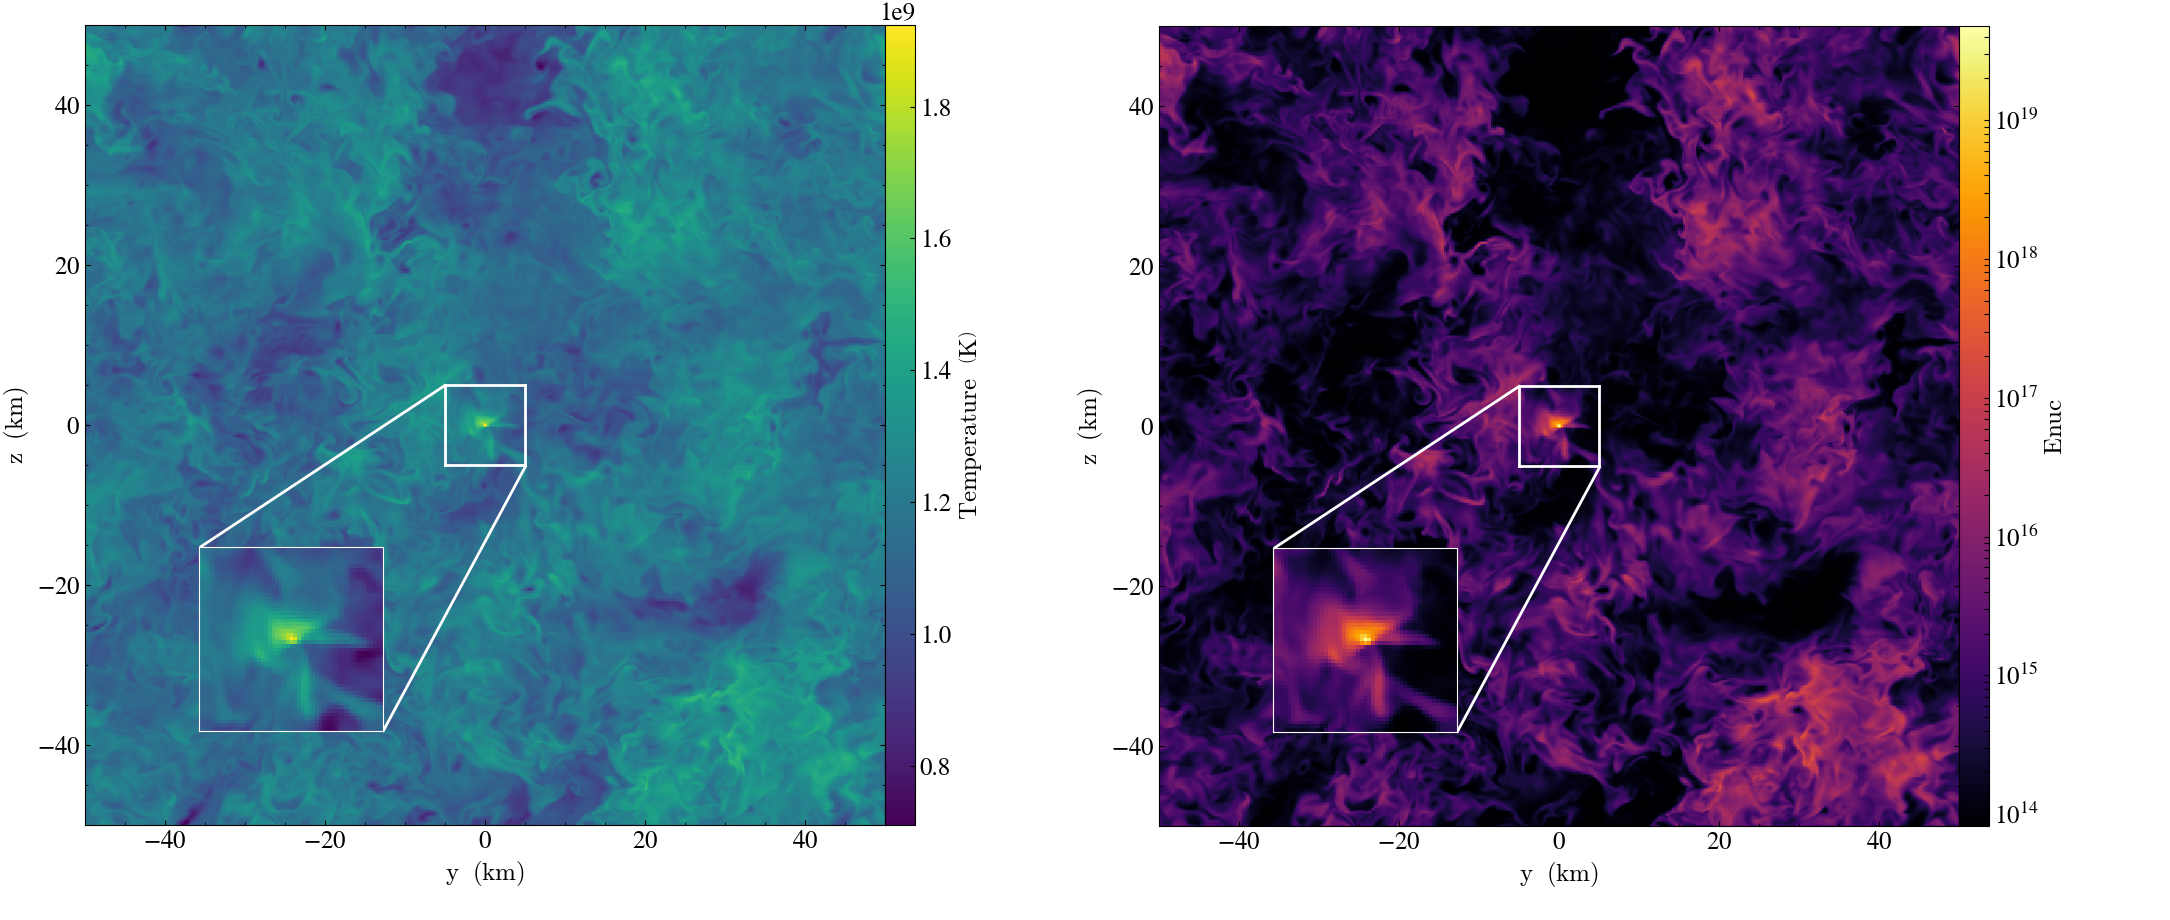
\includegraphics[width=1.0\textwidth]{combined_slice_carbon.png}
\centering
\caption[Slice plots of temperature and specific nuclear energy generation rate, through the maximum temperature in the $z$-$y$ plane, for the $512^3$ run]{Slice plots of temperature and specific nuclear energy generation rate from the C/O run, through the x-axis in the $z$-$y$ plane, for the $512^3$. Each is centered about the hot spot just before leading into a detonation.}
\label {fig:temp_enuc}

\end{figure}
\end{center}

An important implication of these runs is that detonation of carbon can occur in the distributed burning regime through our turbulence mechanism. This is especially important since the Zel'dovich gradient mechanism has been the leading mechanism explaining spontaneous detonation initiation in SNe Ia. Although not wrong, it lacks the physics of turbulence which we know must play a role in the DD channel. From these results, we can now utilize our new mechanism to explore other parameters within these mergers.

\section{Helium Detonation}

Having now a successful detonation mechanism, incorporating helium is a natural next step. As explained before, the detonation of the helium layer of the primary WD opens up the parameter space of how the carbon core can be detonated. Previous work done by Holcomb and collaborators determined tight constraints with regards to temperature, density, and critical length scales for helium burning based upon the Zel'dovich gradient mechanism \cite{holcomb}. They performed one-dimensional hydrodynamic simulations with various initial conditions similar to that which can be modeled with SNe Ia progenitor models. With a turbulently-driven detonation mechanism, we now can perform three-dimensional hydrodynamic simulations and explore the constraints previously modeled.

\section{Simulation Methodology}

Computational tools were used to analyze the physics of turbulence. FLASH, a multiphysics multiscale code built for high-energy density physics, was used to execute three-dimensional hydrodynamic simulations. The hydrodynamics solver used in this case was the split piece-wise parabolic method (PPM). The Helmholtz equation of state was used to incorporate the contributions from nuclei, electrons, blackbody photons, electron-degeneracy, and relativistic effects \cite{timmeswoosley92}. Since this work is only considering a small number of nuclear species, a 19-isotope network was used \cite{weaveretal78}, \cite{timmes99}.

In all, 18 simulations were conducted. Each one had a domain size of $L$ = 100 km, simulated in a fully-periodic box. Spatial resolution ranged from $128^3$ ($L$), $256^3$ ($M$), and $512^3$ ($H$) cells, on a uniform grid. Within each resolution, the parameter space of density and nuclear composition was explored. Densities were set to $10^5$ (LowDen) and $10^6$ (HighDen) g cm$^{-3}$. Initial helium abundance varied from 100\% (PureHe), 25\% (MedHe), and 10\% (MinHe). Carbon and oxygen took up the remaining portion with an assumed equal ratio to one another for each simulation. Initial temperature in all simulations began at $10^8$ K.

Simulations begin with all the fluid having zero velocity. A large-scale stochastic forcing routine is then used as a stirring mechanism to increase the momentum of the simulation. Each simulation runs until the RMS velocities reach a stable value, indicating that it has reached steady-state turbulence. At this point, the simulations are restarted with nuclear burning turned on and are continued to determine whether detonation will occur. Detonation was classified as the time where helium abundance dropped by 10\% of initial value.

\section{Simulation Results}

Slice plots were generated for temperature and specific nuclear burning using the highest resolution models, $512^3$. A snap shot is taken at the time when the detonation has initiated, with the box centered about the point of maximum temperature, which, owing to the extreme sensitivity of the rates to temperature, is also the point of maximum nuclear burning. At this angle, one is looking through the $x$-axis on the $z$-$y$ plane. Each slice plot has an inset which is zoomed in on the hotspot.

Figure 2.2 shows the slice plots for the MinHeLowDen\_H run, which has a $v_{\rm rms} = 1.26 \times 10^8$ cm s$^{-1}$. For all resolutions, these runs fully detonated helium but saw an increase in carbon abundance, while keeping oxygen almost steady. This implies that the helium was burnt off through the triple-alpha process into carbon. Carbon abundances showed no signs of coming to a detonation.

Figure 2.3 shows the slice plots for the MedHeLowDen\_H run, which has a $v_{\rm rms} = 1.28 \times 10^8$ cm s$^{-1}$. Similar to the previous set of parameters, these runs also saw complete detonation of helium with an increase in carbon, while keeping oxygen steady. This also implies that the triple-alpha process fused most of the helium into carbon, while showing no signs of a carbon detonation.

Figure 2.4 shows the slice plots for the PureHeLowDen\_H run. None of these runs, at all resolutions, detonated. However, helium is seen to also burn into carbon through the triple-alpha process. The slice plots are of the last time step recorded, which has a $v_{\rm rms} = 1.25 \times 10^8$ cm s$^{-1}$. A detonation may be observed if simulations ran long enough but this will explored in more detail in future work.

Figure 2.5 shows the slice plots for the MinHeHighDen\_H run, which has a $v_{\rm rms} = 1.22 \times 10^8$ cm s$^{-1}$. All resolutions of these runs saw a detonation of helium and then of carbon shortly afterwards. They also see a rise in oxygen, which implies that on top of the traditional triple-alpha process occuring, an additional alpha capture on carbon occurs to fuse into oxygen.

Figure 2.6 shows the slice plots for the MedHeHighDen\_H run, which has a $v_{\rm rms} = 5.82 \times 10^7$ cm s$^{-1}$. These runs also show complete detonation of helium and carbon with some formation of oxygen, with indications that heavier elements must have been formed post-detonation.

Figure 2.7 shows the slice plots for the PureHeHighDen\_H run, which has a $v_{\rm rms} = 1.25 \times 10^8$ cm s$^{-1}$. These runs see an almost full detonation of helium, with the abundance ratio falling sharply from 100\% to 20\%. At the onset of detonation, carbon abundance rises from \%0 to near 17.5\%, then immediately fully detonates. Oxygen remains steadily at \%0, indicating again that heavier elements have been formed.

\section{Conclusion}

This body of work confirms that turbulently-driven detonation can occur with various abundance levels of helium, carbon, and oxygen. More specifically, the critical temperature for carbon detonation is robustly a factor of $\sim 2-3$ times lower than theorized from previous studies based upon Zel'dovich. Opening up the parameter space of initial conditions for possible detonation scenarios has been an ongoing endeavour for many decades. With newer observational datasets such as \textit{Gaia}, we can now put constraints on our models and also put our focus on specific channels that match these observations. Further work includes exploring more abundance ratios, higher resolutions, and incorporating more in-depth species networks that would allow us to better understand the nucleosynthesis in these simulations.

\begin{comment}
\subsubsection{Column math mode}

Both the \latex\ tabular and \aastex\ deluxetable require an argument to
define the alignment and number of columns.  The most common values are
``c'', ``l'' and ``r'' for \underline{c}enter, \underline{l}eft, and
\underline{r}ight justification.  If these values are capitalized, e.g.
``C'', ``L'', or ``R'', then that specific column will automatically be in math
mode meaning that \$s are not required.  Note that having embedded dollar
signs in the table does not affect the output. 

\subsubsection{Decimal alignment}

Aligning a column by the decimal point can be difficult with only center,
left, and right justification options.  It is possible to use phantom calls
in the data, e.g. {\tt\string\phn}, to align columns by hand but this can
be tedious in long or complex tables.  To address this \aastex\ introduces
the {\tt\string\decimals} command and a new column justification option,
``D'', to align data in that column on the decimal.  In deluxetable the
{\tt\string\decimals} command is invoked before the {\tt\string\startdata}
call but can be anywhere in \latex's tabular environment.  

Two other important thing to note when using decimal alignment is that each
decimal column \textit{must end with a space before the ampersand}, e.g.
``\&\&'' is not allowed.  Empty decimal columns are indicated with a decimal,
e.g. ``.''.  Do not use deluxetable's {\tt\string\nodata} command.

The ``D'' alignment token works by splitting the column into two parts on the
decimal.  While this is invisible to the user one must be aware of how it
works so that the headers are accounted for correctly.  All decimal column
headers need to span two columns to get the alignment correct. This can be
done with a multicolumn call, e.g {\tt\string\multicolumn2c\{\}} or
{\tt\string\multicolumn\{2\}\{c\}\{\}}, or use the new
{\tt\string\twocolhead\{\}} command in deluxetable.  Since \latex\ is
splitting these columns into two it is important to get the table width
right so that they appear joined on the page.  You may have to run the
\latex\ compiler twice to get it right.  

\subsubsection{Automatic column header numbering} \label{subsubsec:autonumber}

The command {\tt\string\colnumbers} can be included to automatically number
each column as the last row in the header. Per the AAS Journal table format
standards, each column index numbers will be surrounded by parentheses. In
a \latex\ tabular environment the {\tt\string\colnumbers} should be invoked
at the location where the author wants the numbers to appear, e.g. after
the last line of specified table header rows. In deluxetable this command
has to come before {\tt\string\startdata}.  {\tt\string\colnumbers} will
not increment for columns hidden by the ``h'' command, see Section
\ref{subsubsec:hide}. 

Note that when using decimal alignment in a table the command 
{\tt\string\decimalcolnumbers} must be used instead of 
{\tt\string\colnumbers} and {\tt\string\decimals}. 

\subsubsection{Hiding columns} \label{subsubsec:hide}

Entire columns can be \underline{h}idden from display simply by changing
the specified column identifier to ``h''.  In the \latex\ tabular environment
this column identifier conceals the entire column including the header
columns.   In \aastex's deluxetables the header row is specifically
declared with the {\tt\string\tablehead} call and each header column is
marked with {\tt\string\colhead} call.  In order to make a specific header
disappear with the ``h'' column identifier in deluxetable use 
{\tt\string\nocolhead} instead to suppress that particular column header.

Authors can use this option in many different ways.  Since column data can
be easily suppressed authors can include extra information and hid it
based on the comments of co-authors or referees.  For wide tables that will
have a machine readable version, authors could put all the information in
the \latex\ table but use this option to hid as many columns as needed until
it fits on a page. This concealed column table would serve as the
example table for the full machine readable version.  Regardless of how
columns are obscured, authors are responsible for removing any unneeded
column data or alerting the editorial office about how to treat these
columns during production for the final typeset article.

Table \ref{tab:messier} provides some basic information about the first ten
Messier Objects and illustrates how many of these new features can be used
together.  It has automatic column numbering, decimal alignment of the
distances, and one concealed column.  The Common name column
is the third in the \latex\ deluxetable but does not appear when the article
is compiled. This hidden column can be shown simply by changing the ``h'' in
the column identifier preamble to another valid value.  This table also
uses {\tt\string\tablenum} to renumber the table because a \latex\ tabular
table was inserted before it.

\begin{deluxetable*}{cchlDlc}
\tablenum{1}
\tablecaption{Fun facts about the first 10 messier objects\label{tab:messier}}
\tablewidth{0pt}
\tablehead{
\colhead{Messier} & \colhead{NGC/IC} & \nocolhead{Common} & \colhead{Object} &
\multicolumn2c{Distance} & \colhead{} & \colhead{V} \\
\colhead{Number} & \colhead{Number} & \nocolhead{Name} & \colhead{Type} &
\multicolumn2c{(kpc)} & \colhead{Constellation} & \colhead{(mag)}
}
\decimalcolnumbers
\startdata
M1 & NGC 1952 & Crab Nebula & Supernova remnant & 2 & Taurus & 8.4 \\
M2 & NGC 7089 & Messier 2 & Cluster, globular & 11.5 & Aquarius & 6.3 \\
M3 & NGC 5272 & Messier 3 & Cluster, globular & 10.4 & Canes Venatici &  6.2 \\
M4 & NGC 6121 & Messier 4 & Cluster, globular & 2.2 & Scorpius & 5.9 \\
M5 & NGC 5904 & Messier 5 & Cluster, globular & 24.5 & Serpens & 5.9 \\
M6 & NGC 6405 & Butterfly Cluster & Cluster, open & 0.31 & Scorpius & 4.2 \\
M7 & NGC 6475 & Ptolemy Cluster & Cluster, open & 0.3 & Scorpius & 3.3 \\
M8 & NGC 6523 & Lagoon Nebula & Nebula with cluster & 1.25 & Sagittarius & 6.0 \\
M9 & NGC 6333 & Messier 9 & Cluster, globular & 7.91 & Ophiuchus & 8.4 \\
M10 & NGC 6254 & Messier 10 & Cluster, globular & 4.42 & Ophiuchus & 6.4 \\
\enddata
\tablecomments{This table ``hides'' the third column in the \latex\ when compiled.
The Distance is also centered on the decimals.  Note that when using decimal
alignment you need to include the {\tt\string\decimals} command before
{\tt\string\startdata} and all of the values in that column have to have a
space before the next ampersand.}
\end{deluxetable*}

\subsubsection{Splitting a table into multiple horizontal components}

Since the AAS Journals are now all electronic with no print version there is
no reason why tables can not be as wide as authors need them to be.
However, there are some artificial limitations based on the width of a
print page.  The old way around this limitation was to rotate into 
landscape mode and use the smallest available table font
sizes, e.g. {\tt\string\tablewidth}, to get the table to fit.
Unfortunately, this was not always enough but now along with the hide column
option outlined in Section \ref{subsubsec:hide} there is a new way to break
a table into two or three components so that it flows down a page by
invoking a new table type, splittabular or splitdeluxetable. Within these
tables a new ``B'' column separator is introduced.  Much like the vertical
bar option, ``$\vert$'', that produces a vertical table lines 
the new ``B'' separator indicates where to \underline{B}reak
a table.  Up to two ``B''s may be included.

Table 2 % \ref{tab:deluxesplit} this freaks it out when it is used!
shows how to split a wide deluxetable into three parts with
the {\tt\string\splitdeluxetable} command.  The {\tt\string\colnumbers}
option is on to show how the automatic column numbering carries through the
second table component, see Section \ref{subsubsec:autonumber}.

\begin{splitdeluxetable*}{lccccBcccccBcccc}
\tabletypesize{\scriptsize}
\tablewidth{0pt} 
\tablenum{5}
\tablecaption{Measurements of Emission Lines: two breaks \label{tab:deluxesplit}}
\tablehead{
\colhead{Model} & \colhead{Component}& \colhead{Shift} & \colhead{FWHM} &
\multicolumn{10}{c}{Flux} \\
\colhead{} & \colhead{} & \colhead{($\rm
km~s^{-1}$)}& \colhead{($\rm km~s^{-1}$)} & \multicolumn{10}{c}{($\rm
10^{-17}~erg~s^{-1}~cm^{-2}$)} \\
\cline{5-14}
\colhead{} & \colhead{} &
\colhead{} & \colhead{} & \colhead{Ly$\alpha$} & \colhead{N\,{\footnotesize
V}} & \colhead{Si\,{\footnotesize IV}} & \colhead{C\,{\footnotesize IV}} &
\colhead{Mg\,{\footnotesize II}} & \colhead{H$\gamma$} & \colhead{H$\beta$}
& \colhead{H$\alpha$} & \colhead{He\,{\footnotesize I}} &
\colhead{Pa$\gamma$}
} 
\colnumbers
\startdata 
{       }& BELs& -97.13 &    9117$\pm      38$&    1033$\pm      33$&$< 35$&$<     166$&     637$\pm      31$&    1951$\pm      26$&     991$\pm 30$&    3502$\pm      42$&   20285$\pm      80$&    2025$\pm     116$& 1289$\pm     107$\\ 
{Model 1}& IELs& -4049.123 & 1974$\pm      22$&    2495$\pm      30$&$<     42$&$<     109$&     995$\pm 186$&      83$\pm      30$&      75$\pm      23$&     130$\pm      25$& 357$\pm      94$&     194$\pm      64$& 36$\pm      23$\\
{       }& NELs& \nodata &     641$\pm       4$&     449$\pm 23$&$<      6$&$<       9$&       --            &     275$\pm      18$& 150$\pm      11$&     313$\pm      12$&     958$\pm      43$&     318$\pm 34$& 151$\pm       17$\\
\hline
{       }& BELs& -85 &    8991$\pm      41$& 988$\pm      29$&$<     24$&$<     173$&     623$\pm      28$&    1945$\pm 29$&     989$\pm      27$&    3498$\pm      37$&   20288$\pm      73$& 2047$\pm     143$& 1376$\pm     167$\\
{Model 2}& IELs& -51000 &    2025$\pm      26$& 2494$\pm      32$&$<     37$&$<     124$&    1005$\pm     190$&      72$\pm 28$&      72$\pm      21$&     113$\pm      18$&     271$\pm      85$& 205$\pm      72$& 34$\pm      21$\\
{       }& NELs& 52 &     637$\pm      10$&     477$\pm 17$&$<      4$&$<       8$&       --            &     278$\pm      17$& 153$\pm      10$&     317$\pm      15$&     969$\pm      40$&     325$\pm 37$&
     147$\pm       22$\\
\enddata
\tablecomments{This is an example of how to split a deluxetable. You can
split any table with this command into two or three parts.  The location of
the split is given by the author based on the placement of the ``B''
indicators in the column identifier preamble.  For more information please
look at the new \aastex\ instructions.}
\end{splitdeluxetable*}

\subsection{Figures\label{subsec:figures}}

%% The "ht!" tells LaTeX to put the figure "here" first, at the "top" next
%% and to override the normal way of calculating a float position
\begin{figure}[ht!]
\plotone{cost.pdf}
\caption{The subscription (squares) and author publication (asterisks) 
costs from 1991 to 2013. Subscription cost are on the left Y axis while
the author costs are on the right Y axis. All numbers in US dollars and
adjusted for inflation. The author charges also account for the change
from page charges to digital quanta in April 2011.  \label{fig:general}}
\end{figure}

Authors can include a wide number of different graphics with their articles
but encapsulated postscript (EPS) or portable document format (PDF) are
encouraged. These range from general figures all authors are familiar with
to new enhanced graphics that can only be fully experienced in HTML.  The
later include figure sets, animations and interactive figures.  All
enhanced graphics require a static two dimensional representation in the
manuscript to serve as the example for the reader. All figures should
include detailed and descriptive captions.  These captions are absolutely
critical for readers for whom the enhanced figure is inaccessible either
due to a disability or offline access.  This portion of the article
provides examples for setting up all these types in with the latest version
of \aastex.

\subsection{General figures\label{subsec:general}}

\aastex\ has a {\tt\string\plotone} command to display a figure consisting
of one EPS/PDF file.  Figure \ref{fig:general} is an example which shows
the approximate changes in the subscription costs and author publication
charges from 1991 to 2013 in the AAS Journals.  For a general figure
consisting of two EPS/PDF files the {\tt\string\plottwo} command can be
used to position the two image files side by side.

Both {\tt\string\plotone} and {\tt\string\plottwo} take a
{\tt\string\caption} and an optional {\tt\string\figurenum} command to
specify the figure number\footnote{It is better to not use
{\tt\string\figurenum} and let LaTeX auto-increment all the figures. If you
do use this command you need to mark all of them accordingly.}.  Each is
based on the {\tt\string graphicx} package command,
{\tt\string\includegraphics}.  Authors are welcome to use
{\tt\string\includegraphics} along with its optional arguments that control
the height, width, scale, and position angle of a file within the figure.
More information on the full usage of {\tt\string\includegraphics} can be
found at \break
\url{https://en.wikibooks.org/wiki/LaTeX/Importing\_Graphics\#Including\_graphics}.

\subsection{Grid figures}

Including more than two EPS/PDF files in a single figure call can be tricky to
easily format.  To make the process easier for authors \aastex\ v6 offers
{\tt\string\gridline} which allows any number of individual EPS/PDF file
calls within a single figure.  Each file cited in a {\tt\string\gridline}
will be displayed in a row.  By adding more {\tt\string\gridline} calls an
author can easily construct a matrix X by Y individual files as a
single general figure.

For each {\tt\string\gridline} command a EPS/PDF file is called by one of
four different commands.  These are {\tt\string\fig},
{\tt\string\rightfig}, {\tt\string\leftfig}, and {\tt\string\boxedfig}.
The first file call specifies no image position justification while the
next two will right and left justify the image, respectively.  The
{\tt\string\boxedfig} is similar to {\tt\string\fig} except that a box is
drawn around the figure file when displayed. Each of these commands takes
three arguments.  The first is the file name.  The second is the width that
file should be displayed at.  While any natural \latex\ unit is allowed, it
is recommended that author use fractional units with the
{\tt\string\textwidth}.  The last argument is text for a subcaption.

Figure \ref{fig:pyramid} shows an inverted pyramid of individual
figure constructed with six individual EPS files using the
{\tt\string\gridline} option.

\begin{figure*}
\gridline{\fig{V2491_Cyg.pdf}{0.3\textwidth}{(a)}
          \fig{HV_Cet.pdf}{0.3\textwidth}{(b)}
          \fig{LMC_2009.pdf}{0.3\textwidth}{(c)}
          }
\gridline{\fig{RS_Oph.pdf}{0.3\textwidth}{(d)}
          \fig{U_Sco.pdf}{0.3\textwidth}{(e)}
          }
\gridline{\fig{KT_Eri.pdf}{0.3\textwidth}{(f)}}
\caption{Inverted pyramid figure of six individual files. The nova are
(a) V2491 Cyg, (b) HV Cet, (c) LMC 2009, (d) RS Oph, (e) U Sco, and (f) 
KT Eri. These individual figures are taken from \citet{2011ApJS..197...31S}.
\label{fig:pyramid}}
\end{figure*}

\subsection{Enhanced graphics}

Enhanced graphics have an example figure to serve as an example for the
reader and the full graphical item available in the published HTML article.
This includes Figure sets, animations, and interactive figures. The 
Astronomy Image Explorer (\url{http://www.astroexplorer.org/}) provides 
access to all the figures published in the AAS Journals since they offered
an electronic version which was in the mid 1990s. You can filter image
searches by specific terms, year, journal, or type. The type filter is 
particularly useful for finding all published enhanced graphics. As of
June 2019 there are over 3000 videos, 1000 figure sets, and 65 interactive
figures. The next sections describe how to include these types of graphics
in your own manuscripts.

\subsubsection{Figure sets}

The grid commands given above works great for a limited set of individual
figure files but what do you do if you have many 10s or 100s or even 1000s of
individual figure files? Figure sets represents a virtual flip book of a
large group of similar style figures.  The derived PDF article will only
shows an example figure while the enhanced content is available in the
figure set in the HTML edition.  The advantage of a figure set gives the
reader the ability to easily sort through a large collection to find
individual component figures.  The advantage to the author is that grouping
similar figures into a figure set can result in significant cost savings in
terms of reduced publication charges, see Appendix B. All of the figure set
components, along with their html framework, are also available to the reader
for download in a single .tar.gz package.

Special \latex\ mark up is required to create a figure set.  Prior to
\aastex\ v6 the underlying mark up commands had to be inserted by hand
but is now included.  Note that when an article with figure set is compiled
in \latex\ none of the component figures are shown and a floating Figure
Set caption will appear in the resulting PDF.

\figsetstart
\figsetnum{4}
\figsettitle{Swift X-ray light curves}

\figsetgrpstart
\figsetgrpnum{1.1}
\figsetgrptitle{KT Eri}
\figsetplot{KT_Eri.pdf}
\figsetgrpnote{The Swift/XRT X-ray light curve for the first year after
outburst of KT Eri.}
\figsetgrpend

\figsetgrpstart
\figsetgrpnum{1.2}
\figsetgrptitle{RS Oph}
\figsetplot{RS_Oph.pdf}
\figsetgrpnote{The Swift/XRT X-ray light curve for the first year after
outburst of RS Oph.}
\figsetgrpend

\figsetgrpstart
\figsetgrpnum{1.3}
\figsetgrptitle{U Sco}
\figsetplot{U_Sco.pdf}
\figsetgrpnote{The Swift/XRT X-ray light curve for the first year after
outburst of U Sco.}
\figsetgrpend

\figsetgrpstart
\figsetgrpnum{1.4}
\figsetgrptitle{V2491 Cyg}
\figsetplot{V2491_Cyg.pdf}
\figsetgrpnote{The Swift/XRT X-ray light curve for the first year after
outburst of V2491 Cyg.}
\figsetgrpend

\figsetgrpstart
\figsetgrpnum{1.5}
\figsetgrptitle{Nova LMC 2009}
\figsetplot{LMC_2009.pdf}
\figsetgrpnote{The Swift/XRT X-ray light curve for the first year after
outburst of nova LMC 2009.}
\figsetgrpend

\figsetgrpstart
\figsetgrpnum{1.6}
\figsetgrptitle{HV Cet}
\figsetplot{HV_Cet.pdf}
\figsetgrpnote{The Swift/XRT X-ray light curve for the first year after
outburst of HV Cet.}
\figsetgrpend

\figsetend

\begin{figure}
\plotone{KT_Eri.pdf}
\caption{The Swift/XRT X-ray light curve for the first year after
outburst of the suspected recurrent nova KT Eri. At a maximum count rate of 
328 ct/s, KT Eri was the brightest nova in X-rays observed to date. All 
the component figures (6) are available in the Figure Set. Note that
these components that are {\bf not} shown in the compiled pdf. The figure
set consists of the same figures as shown in Figure \ref{fig:pyramid}. 
The example figure shown for figure sets can be one component or many. 
\label{fig:fig4}}
\end{figure}

Authors are encouraged to use an online tool at
\url{http://authortools.aas.org/FIGSETS/make-figset.html} to generate their
own specific figure set mark up to incorporate into their \latex\ articles.

\subsubsection{Animations \label{animation}}

Authors may, and are in fact encouraged, to include animations in their
manuscripts. The video will stream inline with the published article and
also be available for download.  When writing the manuscript, a stand alone
figure is necessary to serve as an example for the reader.  Ideally, this
is a single still frame from the animation but in some case the animation
may only represent a small portion of the example figure, say one many
panels as shown in Figure \ref{fig:video}. Regardless, it is very
important that the author provide descriptive text in the figure caption
including start and stop times and the video duration. Authors should
review the AAS animation guidelines in the graphics guide at
\url{https://journals.aas.org/graphics-guide/#animations}.

\begin{figure}
\begin{interactive}{animation}{movie.mp4}
\plotone{f4.pdf}
\end{interactive}
\caption{Figure 1 from \citet{2018ApJ...868L..33L}. AIA 171\AA (a,b), 
AIA 131\AA (c), and AIA 304\AA images are shown. The red rectangle 
in (a) shows the field of view of the other panels. An animation of 
panels (b-d) is available. It covers 8 hours of observing beginning 
at 01:00 UT on 2012 January 19. The video duration is 20 seconds. 
\label{fig:video}}
\end{figure}

Animations and interactive figures (Section \ref{sec:interactive}) should 
use the {\tt\string\begin{interactive}} environment in the figure call. This 
environment
places a blue border around the figure to indicate that the figure is 
enhanced in the published HTML article. The
command also serves to alert the publisher what files are used to generate
the dynamic HTML content. {\tt\string\interactive} takes two arguments. The
first details the type and currently only three are allowed. The types are
{\tt\string js} for generic javascript interactive figures, 
{\tt\string animation} for inline videos, and 
{\tt\string timeseries} for interactive light curves produced
by astropy \citet{2013A&A...558A..33A}\footnote{To be release in the 
summer of 2019}. If these types are not provide the compiler will issue an
error and quit. The second argument is the file that produces the enhanced
feature in the HTML article.

\subsubsection{Interactive figures \label{sec:interactive}}

Interactive figures give the reader the ability to manipulate the
information contained in an image which can add clarity or help further the
author's narrative.  These figures consist of two parts, a static 
representative figure for the manuscript and the dynamic javascript plus
HTML framework that allows for interactive control.

An example of an interactive figure is a 3D model.
The underlying figure is a X3D file while x3dom.js is the javascript driver
that displays it. An author created interface is added via a html wrapper.
The first 3D model published by the AAS Journals using this technique was
\citet{2014ApJ...793..127V}.  

Figure \ref{fig:interactive} provides an interactive example which can be
run locally to demonstrate how a simple javascript plus html interface
allows a reader to switch between figures. The necessary files for this
particular interactive figure are in the {\tt\string interactive.tar.gz}
file included with this package. Unpack the file and point the browser to
the local html file. In this case, the javascript that runs the interactive
buttons is embedded in the html file but it could just as easily be calls
to external javascript libraries. Ideally, the javascript should be
included with the submitted package of interactive files to minimize
external dependencies within the published article.

\begin{figure}
\begin{interactive}{js}{interactive.tar.gz}
\plotone{f5.pdf}
\end{interactive}
\caption{Figure 4 from \citet{2018AJ....156...82C}. \emph{Upper panel}: the
cumulative median observing time to measure the $3\sigma$ RV masses of TESS
planets as a function of host star spectral type and up to $10^3$ hours.
The \emph{dashed blue curves} represent the results from the optical
spectrograph whereas the \emph{solid red curves} represent the near-IR
spectrograph. \emph{Lower panel}: the time derivative of the cumulative
observing time curves used to indicate the RV planet detection efficiency.
The \emph{horizontal dashed line} highlights the value of the detection
efficiency at 20 hours per detection.  Note that unlike the lower panels,
the upper panels do not share a common ordinate due to the differing number
of planet detections around stars in each spectral type bin. The
interactive version has two buttons that allows one to turn the optical and
NIR layers. \label{fig:interactive}}
\end{figure}

Authors should consult the online tutorials at 
\url{https://journals.aas.org/graphics-guide/#interactive_figures}
for more information on what is currently supported and links to 
tutorials and examples.

\section{Displaying mathematics} \label{sec:displaymath}

The most common mathematical symbols and formulas are in the amsmath
package.  \aastex\ requires this package so there is no need to
specifically call for it in the document preamble.  Most modern \latex\
distributions already contain this package.  If you do not have this
package or the other required packages, revtex4-1, latexsym, graphicx,
amssymb, longtable, and epsf, they can be obtained from 
\url{http://www.ctan.org}

Mathematics can be displayed either within the text, e.g. $E = mc^2$, or
separate from in an equation.  In order to be properly rendered, all inline
math text has to be declared by surrounding the math by dollar signs (\$).

A complex equation example with inline math as part of the explanation
follows.

\begin{equation}
\bar v(p_2,\sigma_2)P_{-\tau}\hat a_1\hat a_2\cdots
\hat a_nu(p_1,\sigma_1) ,
\end{equation}
where $p$ and $\sigma$ label the initial $e^{\pm}$ four-momenta
and helicities $(\sigma = \pm 1)$, $\hat a_i=a^\mu_i\gamma_\nu$
and $P_\tau=\frac{1}{2}(1+\tau\gamma_5)$ is a chirality projection
operator $(\tau = \pm1)$.  This produces a single line formula.  \latex\ will
auto-number this and any subsequent equations.  If no number is desired then
the {\tt\string equation} call should be replaced with {\tt\string displaymath}.

\latex\ can also handle a a multi-line equation.  Use {\tt\string eqnarray}
for more than one line and end each line with a
\textbackslash\textbackslash.  Each line will be numbered unless the
\textbackslash\textbackslash\ is preceded by a {\tt\string\nonumber}
command.  Alignment points can be added with ampersands (\&).  There should be
two ampersands per line. In the examples they are centered on the equal
symbol.

\begin{eqnarray}
\gamma^\mu  & = &
 \left(
\begin{array}{cc}
0 & \sigma^\mu_+ \\
\sigma^\mu_- & 0
\end{array}     \right) ,
 \gamma^5= \left(
\begin{array}{cc}
-1 &   0\\
0 &   1
\end{array}     \right)  , \\
\sigma^\mu_{\pm}  & = &   ({\bf 1} ,\pm \sigma) , 
\end{eqnarray}

\begin{eqnarray}
\hat a & = & \left(
\begin{array}{cc}
0 & (\hat a)_+\\
(\hat a)_- & 0
\end{array}\right), \nonumber \\
(\hat a)_\pm & = & a_\mu\sigma^\mu_\pm 
\end{eqnarray}

%% Putting eqnarrays or equations inside the mathletters environment groups
%% the enclosed equations by letter. For instance, the eqnarray below, instead
%% of being numbered, say, (4) and (5), would be numbered (4a) and (4b).
%% LaTeX the paper and look at the output to see the results.

\section{Revision tracking and color highlighting} \label{sec:highlight}

Authors sometimes use color to highlight changes to their manuscript in
response to editor and referee comments.  In \aastex\ new commands
have been introduced to make this easier and formalize the process. 

The first method is through a new set of editing mark up commands that
specifically identify what has been changed.  These commands are
{\tt\string\added\{<text>\}}, {\tt\string\deleted\{<text>\}}, and
{\tt\string\replaced\{<old text>\}\{<replaced text>\}}. To activate these
commands the {\tt\string trackchanges} option must be used in the
{\tt\string\documentclass} call.  When compiled this will produce the
marked text in red.  The {\tt\string\explain\{<text>\}} can be used to add
text to provide information to the reader describing the change.  Its
output is purple italic font. To see how {\tt\string\added\{<important
added info>\}}, {\tt\string\deleted\{<this can be deleted text>\}},
{\tt\string\replaced\{<old data>\}\{<replaced data>\}}, and \break
{\tt\string\explain\{<text explaining the change>\}} commands will produce
\added{important added information}\deleted{, deleted text, and }
\replaced{old data}{and replaced data,} toggle between versions compiled with
and without the {\tt\string trackchanges} option.\explain{text explaining
the change}

A summary list of all these tracking commands can be produced at the end of
the article by adding the {\tt\string\listofchanges} just before the
{\tt\string\end\{document\}} call.  The page number for each change will be
provided. If the {\tt\string linenumbers} option is also included in the
documentclass call then not only will all the lines in the article be
numbered for handy reference but the summary list will also include the
line number for each change.

The second method does not have the ability to highlight the specific
nature of the changes but does allow the author to document changes over
multiple revisions.  The commands are {\tt\string\edit1\{<text>\}},
{\tt\string\edit2\{<text>\}} and {\tt\string\edit3\{<text>\}} and they
produce {\tt\string<text>} that is highlighted in bold red, italic blue and
underlined purple, respectively.  Authors should use the first command to
\edit1{indicated which text has been changed from the first revision.}  The
second command is to highlight \edit2{new or modified text from a second
revision}.  If a third revision is needed then the last command should be used 
\edit3{to show this changed text}.  Since over 90\% of all manuscripts are
accepted after the 3rd revision these commands make it easy to identify
what text has been added and when.  Once the article is accepted all the
highlight color can be turned off simply by adding the
{\tt\string\turnoffediting} command in the preamble. Likewise, the new commands
{\tt\string\turnoffeditone}, {\tt\string\turnoffedittwo}, and
{\tt\string\turnoffeditthree} can be used to only turn off the 
{\tt\string\edit1\{<text>\}}, {\tt\string\edit2\{<text>\}} and 
{\tt\string\edit3\{<text>\}}, respectively.

Similar to marking editing changes with the {\tt\string\edit} options there
are also the {\tt\string\authorcomments1\{<text>\}}, 
{\tt\string\authorcomments2\{<text>\}} and
{\tt\string\authorcomments3\{<text>\}} commands.  These produce the same
bold red, italic blue and underlined purple text but when the
{\tt\string\turnoffediting} command is present the {\tt\string<text>}
material does not appear in the manuscript.  Authors can use these commands
to mark up text that they are not sure should appear in the final
manuscript or as a way to communicate comments between co-authors when
writing the article.

\section{Software and third party data repository citations} \label{sec:cite}

The AAS Journals would like to encourage authors to change software and
third party data repository references from the current standard of a
footnote to a first class citation in the bibliography.  As a bibliographic
citation these important references will be more easily captured and credit
will be given to the appropriate people.

The first step to making this happen is to have the data or software in
a long term repository that has made these items available via a persistent
identifier like a Digital Object Identifier (DOI).  A list of repositories
that satisfy this criteria plus each one's pros and cons are given at \break
\url{https://github.com/AASJournals/Tutorials/tree/master/Repositories}.

In the bibliography the format for data or code follows this format: \\

\noindent author year, title, version, publisher, prefix:identifier\\

\citet{2015ApJ...805...23C} provides a example of how the citation in the
article references the external code at
\doi{10.5281/zenodo.15991}.  Unfortunately, bibtex does
not have specific bibtex entries for these types of references so the
``@misc'' type should be used.  The Repository tutorial explains how to
code the ``@misc'' type correctly.  The most recent aasjournal.bst file,
available with \aastex\ v6, will output bibtex ``@misc'' type properly.

\acknowledgments

I utilize the adaptive mesh refinement code FLASH 4.0.1. The FLASH software used in this work was in part developed by the DOE NNSA-ASC OASCR Flash Center at the University of Chicago. For plotting and analysis, I have made use of yt \cite {Turk_2011}, \url {http://yt-project.org/}. And a special thanks goes out to Dr. Robert Fisher for his guidance, insight and patience throughout this project.


%% To help institutions obtain information on the effectiveness of their 
%% telescopes the AAS Journals has created a group of keywords for telescope 
%% facilities.
%
%% Following the acknowledgments section, use the following syntax and the
%% \facility{} or \facilities{} macros to list the keywords of facilities used 
%% in the research for the paper.  Each keyword is check against the master 
%% list during copy editing.  Individual instruments can be provided in 
%% parentheses, after the keyword, but they are not verified.

\vspace{5mm}
\facilities{HST(STIS), Swift(XRT and UVOT), AAVSO, CTIO:1.3m,
CTIO:1.5m,CXO}

%% Similar to \facility{}, there is the optional \software command to allow 
%% authors a place to specify which programs were used during the creation of 
%% the manuscript. Authors should list each code and include either a
%% citation or url to the code inside ()s when available.

\software{astropy \citep{2013A&A...558A..33A},  
          Cloudy \citep{2013RMxAA..49..137F}, 
          SExtractor \citep{1996A&AS..117..393B}
          }

%% Appendix material should be preceded with a single \appendix command.
%% There should be a \section command for each appendix. Mark appendix
%% subsections with the same markup you use in the main body of the paper.

%% Each Appendix (indicated with \section) will be lettered A, B, C, etc.
%% The equation counter will reset when it encounters the \appendix
%% command and will number appendix equations (A1), (A2), etc. The
%% Figure and Table counter will not reset.

\appendix

\section{Appendix information}

Appendices can be broken into separate sections just like in the main text.
The only difference is that each appendix section is indexed by a letter
(A, B, C, etc.) instead of a number.  Likewise numbered equations have
the section letter appended.  Here is an equation as an example.

\begin{equation}
I = \frac{1}{1 + d_{1}^{P (1 + d_{2} )}}
\end{equation}

Appendix tables and figures should not be numbered like equations. Instead
they should continue the sequence from the main article body.

\section{Author publication charges} \label{sec:pubcharge}

Finally some information about the AAS Journal's publication charges.
In April 2011 the traditional way of calculating author charges based on 
the number of printed pages was changed.  The reason for the change
was due to a recognition of the growing number of article items that could not 
be represented in print. Now author charges are determined by a number of
digital ``quanta''.  A single quantum is 350 words, one figure, one table,
and one enhanced digital item.  For the latter this includes machine readable
tables, figure sets, animations, and interactive figures.  The current cost
for the different quanta types is available at 
\url{https://journals.aas.org/article-charges-and-copyright/#author_publication_charges}. 
Authors may use the ApJL length calculator to get a {\tt rough} estimate of 
the number of word and float quanta in their manuscript. The calculator 
is located at \url{https://authortools.aas.org/ApJL/betacountwords.html}.

\section{Rotating tables} \label{sec:rotate}

The process of rotating tables into landscape mode is slightly different in
\aastex v6.3. Instead of the {\tt\string\rotate} command, a new environment
has been created to handle this task. To place a single page table in a
landscape mode start the table portion with
{\tt\string\begin\{rotatetable\}} and end with
{\tt\string\end\{rotatetable\}}.

Tables that exceed a print page take a slightly different environment since
both rotation and long table printing are required. In these cases start
with {\tt\string\begin\{longrotatetable\}} and end with
{\tt\string\end\{longrotatetable\}}. Table \ref{chartable} is an
example of a multi-page, rotated table. The {\tt\string\movetabledown}
command can be used to help center extremely wide, landscape tables. The
command {\tt\string\movetabledown=1in} will move any rotated table down 1
inch. 

\begin{longrotatetable}
\begin{deluxetable*}{lllrrrrrrll}
\tablecaption{Observable Characteristics of 
Galactic/Magellanic Cloud novae with X-ray observations\label{chartable}}
\tablewidth{700pt}
\tabletypesize{\scriptsize}
\tablehead{
\colhead{Name} & \colhead{V$_{max}$} & 
\colhead{Date} & \colhead{t$_2$} & 
\colhead{FWHM} & \colhead{E(B-V)} & 
\colhead{N$_H$} & \colhead{Period} & 
\colhead{D} & \colhead{Dust?} & \colhead{RN?} \\ 
\colhead{} & \colhead{(mag)} & \colhead{(JD)} & \colhead{(d)} & 
\colhead{(km s$^{-1}$)} & \colhead{(mag)} & \colhead{(cm$^{-2}$)} &
\colhead{(d)} & \colhead{(kpc)} & \colhead{} & \colhead{}
} 
\startdata
CI Aql & 8.83 (1) & 2451665.5 (1) & 32 (2) & 2300 (3) & 0.8$\pm0.2$ (4) & 1.2e+22 & 0.62 (4) & 6.25$\pm5$ (4) & N & Y \\
{\bf CSS081007} & \nodata & 2454596.5 & \nodata & \nodata & 0.146 & 1.1e+21 & 1.77 (5) & 4.45$\pm1.95$ (6) & \nodata & \nodata \\
GQ Mus & 7.2 (7) & 2445352.5 (7) & 18 (7) & 1000 (8) & 0.45 (9) & 3.8e+21  & 0.059375 (10) & 4.8$\pm1$ (9) & N (7) & \nodata \\
IM Nor & 7.84 (11) & 2452289 (2) & 50 (2) & 1150 (12) & 0.8$\pm0.2$ (4) & 8e+21 & 0.102 (13) & 4.25$\pm3.4$ (4) & N & Y \\
{\bf KT Eri} & 5.42 (14) & 2455150.17 (14) & 6.6 (14) & 3000 (15) & 0.08 (15) & 5.5e+20 & \nodata & 6.5 (15) & N & M \\
{\bf LMC 1995} & 10.7 (16) & 2449778.5 (16) & 15$\pm2$ (17) & \nodata & 0.15 (203) & 7.8e+20  & \nodata & 50 & \nodata & \nodata \\
LMC 2000 & 11.45 (18) & 2451737.5 (18) & 9$\pm2$ (19) & 1700 (20) & 0.15 (203) & 7.8e+20  & \nodata & 50 & \nodata & \nodata \\
{\bf LMC 2005} & 11.5 (21) & 2453700.5 (21) & 63 (22) & 900 (23) & 0.15 (203) & 1e+21 & \nodata & 50  & M (24) & \nodata \\
{\bf LMC 2009a} & 10.6 (25) & 2454867.5 (25) & 4$\pm1$  & 3900 (25) & 0.15 (203)  & 5.7e+20 & 1.19 (26) & 50 & N & Y \\
{\bf SMC 2005} & 10.4 (27) & 2453588.5 (27) & \nodata & 3200 (28) & \nodata & 5e+20  & \nodata & 61 & \nodata & \nodata \\
{\bf QY Mus} & 8.1 (29) & 2454739.90 (29) & 60:  & \nodata & 0.71 (30) & 4.2e+21  & \nodata & \nodata & M & \nodata \\
{\bf RS Oph} & 4.5 (31) & 2453779.44 (14) & 7.9 (14) & 3930 (31) & 0.73 (32) & 2.25e+21 & 456 (33) & 1.6$\pm0.3$ (33) & N (34) & Y \\
{\bf U Sco} & 8.05 (35) & 2455224.94 (35) & 1.2 (36) & 7600 (37) & 0.2$\pm0.1$ (4) & 1.2e+21 & 1.23056 (36) & 12$\pm2$ (4) & N & Y \\
{\bf V1047 Cen} & 8.5 (38) & 2453614.5 (39) & 6 (40) & 840 (38) & \nodata & 1.4e+22  & \nodata & \nodata & \nodata & \nodata \\
{\bf V1065 Cen} & 8.2 (41) & 2454123.5 (41) & 11 (42) & 2700 (43) & 0.5$\pm0.1$ (42) & 3.75e+21 & \nodata & 9.05$\pm2.8$ (42) & Y (42) & \nodata \\
V1187 Sco & 7.4 (44) & 2453220.5 (44) & 7: (45) & 3000 (44) & 1.56 (44) & 8.0e+21 & \nodata & 4.9$\pm0.5$ (44) & N & \nodata \\
{\bf V1188 Sco} & 8.7 (46) & 2453577.5 (46) & 7 (40) & 1730 (47) & \nodata & 5.0e+21  & \nodata & 7.5 (39) & \nodata & \nodata \\
{\bf V1213 Cen} & 8.53 (48) & 2454959.5 (48) & 11$\pm2$ (49) & 2300 (50) & 2.07 (30) & 1.0e+22 & \nodata & \nodata & \nodata & \nodata \\
{\bf V1280 Sco} & 3.79 (51) & 2454147.65 (14) & 21 (52) & 640 (53) & 0.36 (54) & 1.6e+21  & \nodata & 1.6$\pm0.4$ (54) & Y (54) & \nodata \\
{\bf V1281 Sco} & 8.8 (55) & 2454152.21 (55) & 15:& 1800 (56) & 0.7 (57) & 3.2e+21 & \nodata & \nodata & N & \nodata \\
{\bf V1309 Sco} & 7.1 (58) & 2454714.5 (58) & 23$\pm2$ (59) & 670 (60) & 1.2 (30) & 4.0e+21 & \nodata & \nodata & \nodata & \nodata \\
{\bf V1494 Aql} & 3.8 (61) & 2451515.5 (61) & 6.6$\pm0.5$ (61) & 1200 (62) & 0.6 (63) & 3.6e+21  & 0.13467 (64) & 1.6$\pm0.1$ (63) & N & \nodata \\
{\bf V1663 Aql} & 10.5 (65) & 2453531.5 (65) & 17 (66) & 1900 (67) & 2: (68) & 1.6e+22  & \nodata & 8.9$\pm3.6$ (69) & N & \nodata \\
V1974 Cyg & 4.3 (70) & 2448654.5 (70) & 17 (71) & 2000 (19) & 0.36$\pm0.04$ (71) & 2.7e+21  & 0.081263 (70) & 1.8$\pm0.1$ (72) & N & \nodata \\
{\bf V2361 Cyg} & 9.3 (73) & 2453412.5 (73) & 6 (40) & 3200 (74) & 1.2: (75) & 7.0e+21 & \nodata & \nodata & Y (40) & \nodata \\
{\bf V2362 Cyg} & 7.8 (76) & 2453831.5 (76) & 9 (77) & 1850 (78) & 0.575$\pm0.015$ (79) & 4.4e+21  & 0.06577 (80) & 7.75$\pm3$ (77) & Y (81) & \nodata \\
{\bf V2467 Cyg} & 6.7 (82) & 2454176.27 (82) & 7 (83) & 950 (82) & 1.5 (84) & 1.4e+22  & 0.159 (85) & 3.1$\pm0.5$ (86) & M (87) & \nodata \\
{\bf V2468 Cyg} & 7.4 (88) & 2454534.2 (88) & 10: & 1000 (88) & 0.77 (89) & 1.0e+22  & 0.242 (90) & \nodata & N & \nodata \\
{\bf V2491 Cyg} & 7.54 (91) & 2454567.86 (91) & 4.6 (92) & 4860 (93) & 0.43 (94) & 4.7e+21  & 0.09580: (95) & 10.5 (96) & N & M \\
V2487 Oph & 9.5 (97) & 2450979.5 (97) & 6.3 (98) & 10000 (98) & 0.38$\pm0.08$ (98) & 2.0e+21 & \nodata & 27.5$\pm3$ (99) & N (100) & Y (101) \\
{\bf V2540 Oph} & 8.5 (102) & 2452295.5 (102) & \nodata & \nodata & \nodata & 2.3e+21 & 0.284781 (103) & 5.2$\pm0.8$ (103) & N & \nodata \\
V2575 Oph & 11.1 (104) & 2453778.8 (104) & 20: & 560 (104) & 1.4 (105) & 3.3e+21 & \nodata & \nodata & N (105) & \nodata \\
{\bf V2576 Oph} & 9.2 (106) & 2453832.5 (106) & 8: & 1470 (106) & 0.25 (107) & 2.6e+21  & \nodata & \nodata & N & \nodata \\
{\bf V2615 Oph} & 8.52 (108) & 2454187.5 (108) & 26.5 (108) & 800 (109) & 0.9 (108) & 3.1e+21  & \nodata & 3.7$\pm0.2$ (108) & Y (110) & \nodata \\
{\bf V2670 Oph} & 9.9 (111) & 2454613.11 (111) & 15: & 600 (112) & 1.3: (113) & 2.9e+21  & \nodata & \nodata & N (114) & \nodata \\
{\bf V2671 Oph} & 11.1 (115) & 2454617.5 (115) & 8: & 1210 (116) & 2.0 (117) & 3.3e+21  & \nodata & \nodata & M (117) & \nodata \\
{\bf V2672 Oph} & 10.0 (118) & 2455060.02 (118) & 2.3 (119) & 8000 (118) & 1.6$\pm0.1$ (119) & 4.0e+21  & \nodata & 19$\pm2$ (119) & \nodata & M \\
V351 Pup & 6.5 (120) & 2448617.5 (120) & 16 (121) & \nodata & 0.72$\pm0.1$ (122) & 6.2e+21 & 0.1182 (123) & 2.7$\pm0.7$ (122) & N & \nodata \\
{\bf V382 Nor} & 8.9 (124) & 2453447.5 (124) & 12 (40) & 1850 (23) & \nodata & 1.7e+22 & \nodata & \nodata & \nodata & \nodata \\
V382 Vel & 2.85 (125) & 2451320.5 (125) & 4.5 (126) & 2400 (126) & 0.05: (126) & 3.4e+21  & 0.146126 (127) & 1.68$\pm0.3$ (126) & N & \nodata \\
{\bf V407 Cyg} & 6.8 (128) & 2455266.314 (128) & 5.9 (129) & 2760 (129) & 0.5$\pm0.05$ (130) & 8.8e+21 & 15595 (131) & 2.7 (131) & \nodata & Y \\
{\bf V458 Vul} & 8.24 (132) & 2454322.39 (132) & 7 (133) & 1750 (134) & 0.6 (135) & 3.6e+21 & 0.06812255 (136) & 8.5$\pm1.8$ (133) & N (135) & \nodata \\
{\bf V459 Vul} & 7.57 (137) & 2454461.5 (137) & 18 (138) & 910 (139) & 1.0 (140) & 5.5e+21  & \nodata & 3.65$\pm1.35$ (138) & Y (140) & \nodata \\
V4633 Sgr & 7.8 (141) & 2450895.5 (141) & 19$\pm3$ (142) & 1700 (143) & 0.21 (142) & 1.4e+21  & 0.125576 (144) & 8.9$\pm2.5$ (142) & N & \nodata \\
{\bf V4643 Sgr} & 8.07 (145) & 2451965.867 (145) & 4.8 (146) & 4700 (147) & 1.67 (148) & 1.4e+22 & \nodata & 3 (148) & N & \nodata \\
{\bf V4743 Sgr} & 5.0 (149) & 2452537.5 (149) & 9 (150) & 2400 (149) & 0.25 (151) & 1.2e+21 & 0.281 (152) & 3.9$\pm0.3$ (151) & N & \nodata \\
{\bf V4745 Sgr} & 7.41 (153) & 2452747.5 (153) & 8.6 (154) & 1600 (155) & 0.1 (154) & 9.0e+20  & 0.20782 (156) & 14$\pm5$ (154) & \nodata & \nodata \\
{\bf V476 Sct} & 10.3 (157) & 2453643.5 (157) & 15 (158) & \nodata & 1.9 (158) & 1.2e+22  & \nodata & 4$\pm1$ (158) & M (159) & \nodata \\
{\bf V477 Sct} & 9.8 (160) & 2453655.5 (160) & 3 (160) & 2900 (161) & 1.2: (162) & 4e+21  & \nodata & \nodata & M (163) & \nodata \\
{\bf V5114 Sgr} & 8.38 (164) & 2453081.5 (164) & 11 (165) & 2000 (23) & \nodata & 1.5e+21  & \nodata & 7.7$\pm0.7$ (165) & N (166) & \nodata \\
{\bf V5115 Sgr} & 7.7 (167) & 2453459.5 (167) & 7 (40) & 1300 (168) & 0.53 (169) & 2.3e+21  & \nodata & \nodata & N (169) & \nodata \\
{\bf V5116 Sgr} & 8.15 (170) & 2453556.91 (170) & 6.5 (171) & 970 (172) & 0.25 (173) & 1.5e+21 & 0.1238 (171) & 11$\pm3$ (173) & N (174) & \nodata \\
{\bf V5558 Sgr} & 6.53 (175) & 2454291.5 (175) & 125 (176) & 1000 (177) & 0.80 (178) & 1.6e+22  & \nodata & 1.3$\pm0.3$ (176) & N (179) & \nodata \\
{\bf V5579 Sgr} & 5.56 (180) & 2454579.62 (180) & 7: & 1500 (23) & 1.2 (181) & 3.3e+21 & \nodata & \nodata & Y (181) & \nodata \\
{\bf V5583 Sgr} & 7.43 (182) & 2455051.07 (182) & 5: & 2300 (182) & 0.39 (30) & 2.0e+21 & \nodata & 10.5 & \nodata & \nodata \\
{\bf V574 Pup} & 6.93 (183) & 2453332.22 (183) & 13 (184) & 2800 (184) & 0.5$\pm0.1$  & 6.2e+21 & \nodata & 6.5$\pm1$  & M (185) & \nodata \\
{\bf V597 Pup} & 7.0 (186) & 2454418.75 (186) & 3: & 1800 (187) & 0.3 (188) & 5.0e+21  & 0.11119 (189) & \nodata & N (188) & \nodata \\
{\bf V598 Pup} & 3.46 (14) & 2454257.79 (14) & 9$\pm1$ (190) & \nodata & 0.16 (190) & 1.4e+21 & \nodata & 2.95$\pm0.8$ (190) & \nodata & \nodata \\
{\bf V679 Car} & 7.55 (191) & 2454797.77 (191) & 20: & \nodata & \nodata & 1.3e+22  & \nodata & \nodata & \nodata & \nodata \\
{\bf V723 Cas} & 7.1 (192) & 2450069.0 (192) & 263 (2) & 600 (193) & 0.5 (194) & 2.35e+21  & 0.69 (195) & 3.86$\pm0.23$ (196) & N & \nodata \\
V838 Her & 5 (197) & 2448340.5 (197) & 2 (198) & \nodata & 0.5$\pm0.1$ (198) & 2.6e+21  & 0.2975 (199) & 3$\pm1$ (198) & Y (200) & \nodata \\
{\bf XMMSL1 J06} & 12 (201) & 2453643.5 (202) & 8$\pm2$ (202) & \nodata & 0.15 (203) & 8.7e+20 & \nodata & 50 & \nodata & \nodata \\
\enddata
\end{deluxetable*}
\end{longrotatetable}

A handy "cheat sheet" that provides the necessary LaTeX to produce 17 
different types of tables is available at \url{http://journals.aas.org/authors/aastex/aasguide.html#table_cheat_sheet}.

\section{IAU recommendations for nominal units \label{nominal}}

The IAU 2015 resolution B3 defines nominal solar and planetary values by
establishing conversions between solar and planetary values and SI units.
The rational and specifications are given in \citet{2016AJ....152...41P}.
The recommended nominal conversion constants for LaTeX have been
incorporate into v6.3 to help authors follow the IAU resolution.

The general commands take this form:

\vskip12pt
\begin{center}
\begin{tabular}{@{\vrule height 14pt depth 6pt width0pt}lll}
Command&Example&Results\\
\verb+\nom{}+&\verb+\nom{Q}+&\nom{Q}\\
\verb+\Eenom{}+&\verb+\Eenom{Q}+&\Eenom{Q}\\
\verb+\Epnom{}+&\verb+\Epnom{Q}+&\Epnom{Q}\\
\verb+\Jenom{}+&\verb+\Jenom{Q}+&\Jenom{Q}\\
\verb+\Jpnom{}+&\verb+\Jpnom{Q}+&\Jpnom{Q}\\
\end{tabular}
\end{center}
\vskip12pt

which can be used for any units the author requires. Examples of 
the most common uses would be:

\vskip12pt
\begin{tabular}{@{\vrule height 14pt depth 6pt width 0pt}llllp{3in}}
1.&\verb+\nom{(GM)}+& \nom{(GM)} &=& nominal solar mass parameter\\
2.&\verb+\nom{R}+&\nom{R} &=& nominal solar radius\\
3.&\verb+\nom{S}+& \nom{S}&=&  nominal total solar irradiance\\
4.&\verb+\nom{L}+& \nom{L}  &=&nominal solar luminosity\\
\end{tabular}
\vskip12pt

AASTeX v6.3 also contains specific commands for other commonly used 
units. These are:

\vskip24pt
\begin{tabular}{@{\vrule height 14pt depth 6pt width 0pt}llllp{3in}}
1.&\verb+\nomSolarEffTemp+& \nomSolarEffTemp&=& nominal solar effective temperature\\
2.&\verb+\nomTerrEqRadius+&\nomTerrEqRadius  &=& nominal terrestrial
equatorial radius\\
&\verb+\nomTerrPolarRadius+ &\nomTerrPolarRadius &=& nominal
terrestrial polar radius\\
&\verb+\nomTerrEqRadius+&\nomTerrEqRadius&& should be used if equatorial
vs.~polar radius is not explicitly specified.\\
3.&\verb+\nomJovianEqRadius+&\nomJovianEqRadius&=& nominal one-bar equatorial radii of
Jupiter\\
&\verb+\nomJovianPolarRadius+&\nomJovianPolarRadius &=& nominal polar radii of Jupiter\\
&\verb+\nomJovianEqRadius+&\nomJovianEqRadius&& should be used if Jovian equatorial
vs.~polar radius is not explicitly specified.\\
4.&\verb+\nomTerrMass+ &\nomTerrMass &=& nominal terrestrial mass
parameter\\
&\verb+\nomJovianMass+ &\nomJovianMass &=& nominal Jovian mass parameter\\
\end{tabular}
\vskip12pt

All of these commands work equally well in text and math mode.

%% For this sample we use BibTeX plus aasjournals.bst to generate the
%% the bibliography. The sample63.bib file was populated from ADS. To
%% get the citations to show in the compiled file do the following:
%%
%% pdflatex sample63.tex
%% bibtext sample63
%% pdflatex sample63.tex
%% pdflatex sample63.tex

\bibliography{sample63}{}
\bibliographystyle{aasjournal}

%% This command is needed to show the entire author+affiliation list when
%% the collaboration and author truncation commands are used.  It has to
%% go at the end of the manuscript.
%\allauthors

%% Include this line if you are using the \added, \replaced, \deleted
%% commands to see a summary list of all changes at the end of the article.
%\listofchanges
\end{comment}

\end{document}

% End of file `sample63.tex'.
